% Chapter Template

\chapter{Эксперименты в классической задаче} % Main chapter title

\label{ExperimentsClassic} % Change X to a consecutive number; for referencing this chapter elsewhere, use \ref{ChapterX}

\section{Параметры}

Список используемых семейств распределений дан в таблице \ref{table:classic_distribution_family}. Число $a$ для каждого рычага сэмплируется из $\mathcal{N}(0,1)$ (за исключением градиентных бандитов, чтобы продемонстрировать их невосприимичвость к изменению среднего). Списки отдельных экспериментов с применяемыми в них стратегиями даны в таблицах \ref{table:classic_greedy}, \ref{table:classic_positive}, \ref{table:classic_ucb}, \ref{table:classic_gradient_bandits}. Параметры, общие для каждого тестирования, даны в таблице \ref{table:classic_hyperparameters}. Для распределения Коши лучшим считался рычаг с наибольшей медианой. Метрики даны в таблице \ref{table:classic_metrics}. Для каждого распределения и каждой метрики результаты для одной группы стратегий визуализированы на графике. Кроме того, было решено дополнительно изобразить для каждой стратегии и для каждой метрики на одном графике результаты по всем распределениям. Ввиду большой шумности средней награды для $t_2$ результаты были обработаны усредняющим скользящим окном длины 5.

В конце был проведен обзор всех стратегий для различных значений гиперпараметров. Для всех распределений $m_a \sim \mathcal{N}(0,1)$. Для каждой стратегии варьировался один ключевой гиперпараметр, варьирование происходило по значениям
\[
\frac{1}{128}, \frac{1}{64}, \frac{1}{32}, \frac{1}{16}, \frac{1}{8}, \frac{1}{4}, \frac{1}{2}, 1, 2, 4
\]
(для $\epsilon$-greedy значения 2 и 4 не рассматривались). Стратегии для финального тестирования даны в таблице \ref{table:classic_final} 
 
Ввиду долгого выполнения процент оптимальных действий и средняя награда брались по 1000 тестам, при этом количество шагов осталось равным 1000. В случае средней награды бралась средняя награда за все 1000 шагов, в случае оптимального действий брался средний процент за 1000 шагов. Полученные результаты были визуализированы на графике.

\begin{table}
\centering
\renewcommand{\arraystretch}{1.5}
\begin{tabular}{ |m{4cm}||m{2.1cm}|m{6cm}|  }
 \hline
 \multicolumn{3}{|c|}{Список используемых распределений} \\
 \hline
 Распределение & Обозначение & Плотность $p(x)$ \\
 \hline
  Нормальное   &  $t_{\infty} $&  $\frac{1}{\sqrt{2\pi}}e^{\frac{(x-a)^2}{2}}$ \\
 \hline
 Стьюдента с $\nu=3$ нормированное & $t_{3}$ & $\frac{1}{\sqrt{3}} \cdot \frac{2}{\pi \sqrt{3} \left( 1 + \frac{(x-a)^2}{3} \right)^2}$ \\
 \hline
 Стьюдента с $\nu=2.1$ нормированное & $t_{2.1}$ & $\frac{1}{\sqrt{21}} \cdot \frac{\Gamma(1.55)}{\sqrt{2.1 \pi} \Gamma(1.05)} \left( 1 + \frac{(x-a)^2}{2.1} \right)^{-1.55}$ \\
 \hline
 Стьюдента с $\nu=2$ & $t_2$ & $\frac{1}{2\sqrt{2} \left( 1 + \frac{(x-a)^2}{2} \right)^{3/2}}$ \\
 \hline
 Коши & $t_1$ & $\frac{1}{\pi(1+(x-a)^2)}$ \\
 \hline
\end{tabular}
\caption{Список семейств распределений для проверки стратегий в классической задаче о многоруких бандитах. Рычаги каждый раз берутся из одного семейства.}
\label{table:classic_distribution_family}
\end{table}

\begin{table}
\centering
\renewcommand{\arraystretch}{1.3}
\begin{tabular}{ |m{3cm}|m{5cm}|  }
 \hline
 \multicolumn{2}{|c|}{Тест $\epsilon$-greedy} \\
 \hline
 Стратегия & Параметры \\
 \hline
  Жадная   &  $\epsilon = 0, \: \forall a \hook Q_1(a) = 0$ \\
 \hline
 $\epsilon$-жадная & $\epsilon = 0.01, \: \forall a \hook Q_1(a) = 0$ \\
 \hline
 $\epsilon$-жадная & $\epsilon = 0.1, \: \forall a \hook Q_1(a) = 0$ \\
 \hline
\end{tabular}
\caption{Параметры для теста жадной и $\epsilon$-жадной стратегий в классической задаче}
\label{table:classic_greedy}
\end{table}

\begin{table}
\centering
\renewcommand{\arraystretch}{1.3}
\begin{tabular}{ |m{4cm}|m{5cm}|  }
 \hline
 \multicolumn{2}{|c|}{Тест позитивной инициализации} \\
 \hline
 Стратегия & Параметры \\
 \hline
 $\epsilon$-жадная & $\epsilon = 0.1, \: \forall a \hook Q_1(a) = 0$ \\
 \hline
 Жадная оптимистичная & $\epsilon = 0, \: \forall a \hook Q_1(a) = 5$ \\
 \hline
 $\epsilon$-жадная оптимистичная & $\epsilon = 0.1, \: \forall a \hook Q_1(a) = 5$ \\
 \hline
\end{tabular}
\caption{Параметры для теста стратегий с позитивной инициализацией в классической задаче}
\label{table:classic_positive}
\end{table}

\begin{table}
\centering
\renewcommand{\arraystretch}{1.3}
\begin{tabular}{ |m{3cm}|m{4cm}|  }
 \hline
 \multicolumn{2}{|c|}{Тест UCB ($\forall a \hook Q_1(a) = 0$)} \\
 \hline
 Стратегия & Параметры \\
 \hline
 $\epsilon$-жадная & $\epsilon = 0.1$ \\
 \hline
 UCB & $c=2, \, \epsilon=0.001$ \\
 \hline
\end{tabular}
\caption{Параметры для теста UCB}
\label{table:classic_ucb}
\end{table}

\begin{table}
\centering
\renewcommand{\arraystretch}{1.3}
\begin{tabular}{ |m{4cm}|m{6cm}|  }
 \hline
 \multicolumn{2}{|c|}{Тест градиентных бандитов ($\forall a \hook Q_1(a) = 0, \, H_1(a) = 0, \, m_a \sim \mathcal{N}(4,1)$)} \\
 \hline
 Стратегия & Параметры \\
 \hline
 Градиентные бандиты & $\alpha=0.1, \text{baseline} = \bar{R_t}$ \\
 \hline
 Градиентные бандиты & $\alpha=0.1, \text{baseline} = 0$ \\
 \hline
 Градиентные бандиты & $\alpha=0.4, \text{baseline} = \bar{R_t}$ \\
 \hline
 Градиентные бандиты & $\alpha=0.4, \text{baseline} = 0$ \\
 \hline
\end{tabular}
\caption{Параметры для теста градиентных бандитов в классической задаче}
\label{table:classic_gradient_bandits}
\end{table}

\begin{table}
\centering
\renewcommand{\arraystretch}{1.3}
\begin{tabular}{ |m{4cm}|m{2.1cm}|m{2cm}|  }
 \hline
 \multicolumn{3}{|c|}{Гиперпараметры тестов} \\
 \hline
 Гиперпараметр & Обозначение & Значение \\
 \hline
  Число рычагов   &  $n$ &  10 \\
 \hline
 Количество инстансов теста & test\_num & 2000 \\
 \hline
 Количество шагов в инстансе & test\_len & 1000 \\
 \hline
\end{tabular}
\caption{Гиперпараметры для тестирования стратегий в классической задаче}
\label{table:classic_hyperparameters}
\end{table}

\begin{table}
\centering
\renewcommand{\arraystretch}{2}
\begin{tabular}{ |m{4cm}|m{5cm}|  }
 \hline
 \multicolumn{2}{|c|}{Метрики} \\
 \hline
 Название & Формула \\
 \hline
 Средняя награда на шаге $t$ & $\frac{\sum_{i=1}^{test\_num} R_t^{(i)}}{test\_num}$ \\
 \hline
 Средний процент оптимальных действий на шаге $t$ & $\frac{\sum_{i=1}^{test\_num} \bb{I}(A_t^{(i)} = \underset{a}{\arg \max} \, m_a)}{test\_num}$ \\
 \hline
\end{tabular}
\caption{Метрики для проверки эффективности стратегий в классической задаче}
\label{table:classic_metrics}
\end{table}

\begin{table}
\centering
\renewcommand{\arraystretch}{1.3}
\begin{tabular}{ |m{4cm}|m{4cm}|m{4cm}|  }
 \hline
 \multicolumn{3}{|c|}{Стратегии для финального теста} \\
 \hline
 Стратегия & Параметры & Варьирование по \\
 \hline
  $\epsilon$-greedy   &  $\forall a \hook Q_1(a) = 0$ &  $\epsilon$ \\
 \hline
 greedy с оптимистичной инициализацией & $\alpha = 0.1$ & $Q_1(a)$ \\
 \hline
 UCB & $\epsilon = 0.001, \: \forall a \hook Q_1(a) = 0$ & $c$ \\
 \hline
 Gradient bandits & $\text{baseline} = \bar{R_t}$ & $\alpha$ \\
 \hline
\end{tabular}
\caption{Стратегии, их параметры, и параметры, по которым происходит варьирование, для финального тестирования в классической задаче}
\label{table:classic_final}
\end{table}

\section{Результаты}

На всех графиках график средней награды для распределения Коши не имеет смысла ввиду отсутствия у распределения матожидания.

\subsection{$\epsilon$-greedy}
\label{subsec:classic_epsilon_greedy}

$\epsilon$-greedy: Как можно видеть, для $t_2, t_{2.1}, t_3, t_{\infty}$ при увеличении $\epsilon$ до значения $\frac{1}{n} = \frac{1}{10}$ средняя награда и процент оптимальных действий увеличиваются. Для $t_2$ характерны резкие прыжки в средней награде ввиду отсутствия дисперсии. Для $t_1$ процент оптимальных действий значительно ниже других распределений и составляет около $30\%$, более того, оптимальный процент действий для каждой из стратегий примерно одинаков, изменение $\epsilon$ не ведет к изменению процента оптимальных действий для $t_1$. Стоит предположить, что при $\nu \to 0$ процент оптимальных действий $t_{\nu}$ стремится к $\frac{1}{n}$. При положительном $\epsilon$ средняя награда и процент оптимальных действий для $t_3$ и $t_{\infty}$ примерно одинаковы, для $t_2$ эти значения несколько ниже, а вот для $t_{2.1}$, наоборот, стало выше. Для greedy стратегии наблюдается другая картина: метрики для $t_{\infty}$ выше, чем для $t_3$, что можно объяснить тем, что после сжатия $t_3$ его пик стал более острым, и более резких изменений стало меньше, чем у $t_{\infty}$, из-за чего исправлений неправильных выборов рычагов стало меньше. Это же объясняет результат для $t_{2.1}$ -- ввиду большей остроты пика при случайном выборе значения меньше отстоят от матожидания, что дает более хорошее приближение и повышает частоту выбора правильного рычага. Для $t_2$ наоборот, метрики выше, чем у $t_{\infty}$, что объясняется отсутствием дисперсии и более частыми ``далекими'' значениями, что повышает вероятность исправления неправильных выборов рычагов.
\begin{figure}[ht!]
    \centering
    \includegraphics[width=1.1\linewidth]{experiments_classic/eps_greedy/first.png}
    \caption{\label{fig:eps_greedy_1}Значения средней награды и процента оптимального выбора для $\epsilon$-greedy стратегий, сгруппировано по распределениям}
\end{figure}
\begin{figure}[ht!]
    \centering
    \includegraphics[width=1.1\linewidth]{experiments_classic/eps_greedy/second.png}
    \caption{\label{fig:eps_greedy_1}Значения средней награды и процента оптимального выбора для $\epsilon$-greedy стратегий, сгруппировано по стратегиям}
\end{figure}

\subsection{Позитивная инициализация}

Для позитивной инициализации ситуация несколько отличается \ref{fig:optimistic_1}. Оптимистичная жадная стратегия лучше оптимистичной $\epsilon$-greedy и реалистичной $\epsilon$-greedy только для $t_{\infty}$, $t_3$ и $t_{2.1}$, причем для $t_3$ процент оптимальных действий для всех трех стратегий выравнивается к 1000-му шагу. Для $t_{2.1}$ и $t_{\infty}$ оптимистичная жадная стратегия значительно лучше остальных стратегий. Для $t_2$ и $t_1$ средняя награда и процент оптимальных действий для оптимистичной жадной стратегии хуже, чем для остальных стратегий. То есть жадность стратегии и постоянный step-size сильнее влияют на результат, чем позитивная инициализация. При этом для всех распределений для $\epsilon$-greedy оптимистичной и реалистичной стратегий средняя награда и процент оптимальных действий выравниваются, что объясняется маленьким вкладом начальной инициализации на 1000-ом шаге. Кроме того, для $t_{2.1}, t_2, t_1$ и константного step-size наблюдается переобучение: в какой-то момент средняя награда и процент оптимальных действий начинают падать. Такая проблема возникает в силу того, что для константного step-size вклад выбросов не уменьшается со временем, и потому для распределений с тяжелыми хвостами возникает ситуация, когда приход ``выброса'' резко изменяет среднюю награду оптимального действия в отрицательную сторону, и затем это действие выбирается гораздо реже. Аналогично предыдущему эксперименту, для $t_2$ виден разброс в средней награде из-за отсутствия дисперсии.

Если сравнивать распределения на \ref{fig:optimistic_2}, то с уменьшением степеней свободы обе метрики падают. При этом для $t_{2.1}$ высота пика в проценте оптимальных действий на 10-ом шаге выше, чем для $t_{\infty}$, что опять же, можно объяснить большей остротой пика. Результаты для $t_{2}$ намного хуже остальных распределений, аналогично предыдущему пункту, из-за большого разброса значений вследствие отсутствия дисперсии.
\begin{figure}[ht!]
    \centering
    \includegraphics[width=1.1\linewidth]{experiments_classic/positive/first.png}
    \caption{\label{fig:optimistic_1}Значения средней награды и процента оптимального выбора для оптимистичной стратегии в сравнении с $\epsilon$-greedy стратегий для константного step-size, сгруппировано по распределениям. Для $t_{2.1}, t_2, t_1$ видно переобучение}
\end{figure}
\begin{figure}[ht!]
    \centering
    \includegraphics[width=1.1\linewidth]{experiments_classic/positive/second.png}
    \caption{\label{fig:optimistic_2}Значения средней награды и процента оптимального выбора для оптимистичной и $\epsilon$-greedy стратегий для константного step-size, сгруппировано по стратегиям.}
\end{figure}

\subsection{UCB}

Для Upper-Confidence Bound Action Selection на всех распределениях и всех метриках видно, что UCB лучше $\epsilon$-greedy стратегии (пусть для $t_{2.1}$ UCB вырывается вперед только в самом конце) (\ref{fig:ucb_1}). Это можно объяснить тем, что UCB с увеличением уверенности реже производит "исследование" действий. При этом с уменьшением числа степеней свободы средняя награда и процент оптимальных действий при $\nu > 2$ практически не падает, а процент для $\nu = 2$ падает заметно \ref{fig:ucb_2}. Для $t_{\infty}$, $t_3$ и $t_{2.1}$ метрики падают на очень малую величину, позволяющую сказать, что UCB одинаково применимо для этих распределений.
\begin{figure}[ht!]
    \centering
    \includegraphics[width=1.1\linewidth]{experiments_classic/UCB/first.png}
    \caption{\label{fig:ucb_1}Значения средней награды и процента оптимального выбора для UCB в сравнении с $\epsilon$-greedy, сгруппировано по распределениям. UCB лучше $\epsilon$-greedy на всех распределениях}
\end{figure}
\begin{figure}[ht!]
    \centering
    \includegraphics[width=1.1\linewidth]{experiments_classic/UCB/second.png}
    \caption{\label{fig:ucb_2}Значения средней награды и процента оптимального выбора для UCB, сгруппировано по стратегиям.}
\end{figure}

\subsection{Gradient bandits}

Gradient bandits: для всех распределений присутствие baseline повышает значения метрик. Кроме того, значения метрик при $\alpha=0.1$ лучше, чем при $\alpha=0.4$ при заданных распределении и baseline, поскольку изменение $H_t(a)$ и, значит, $\pi_t(a)$, происходит менее резко, и выбросы меньше влияют на результат. С уменьшением $\nu$ разрыв в проценте оптимальных действий для для $\alpha=0.4$ с baseline и $\alpha=0.1$ без baseline сокращается, а для $t_1$ и вовсе почти совпадают, что дает говорить о том, что с уменьшением числа степеней свободы влияние baseline уменьшается. Впрочем, при $\nu \leq 1$ само понятие выборочного среднего как приближение матожидания перестает иметь смысл. Аналогично предыдущим пунктам, для $t_2$ и $t_1$ значение метрик ниже, чем для $t_3$ и $t_{\infty}$. Причем при увеличении $\alpha$ в ситуации с пристусттвием baseline значения метрик для $t_{\infty}$ становятся ниже, чем для $t_3$, при отсутствии baseline ситуация ровно наоборот.
\begin{figure}[ht!]
    \centering
    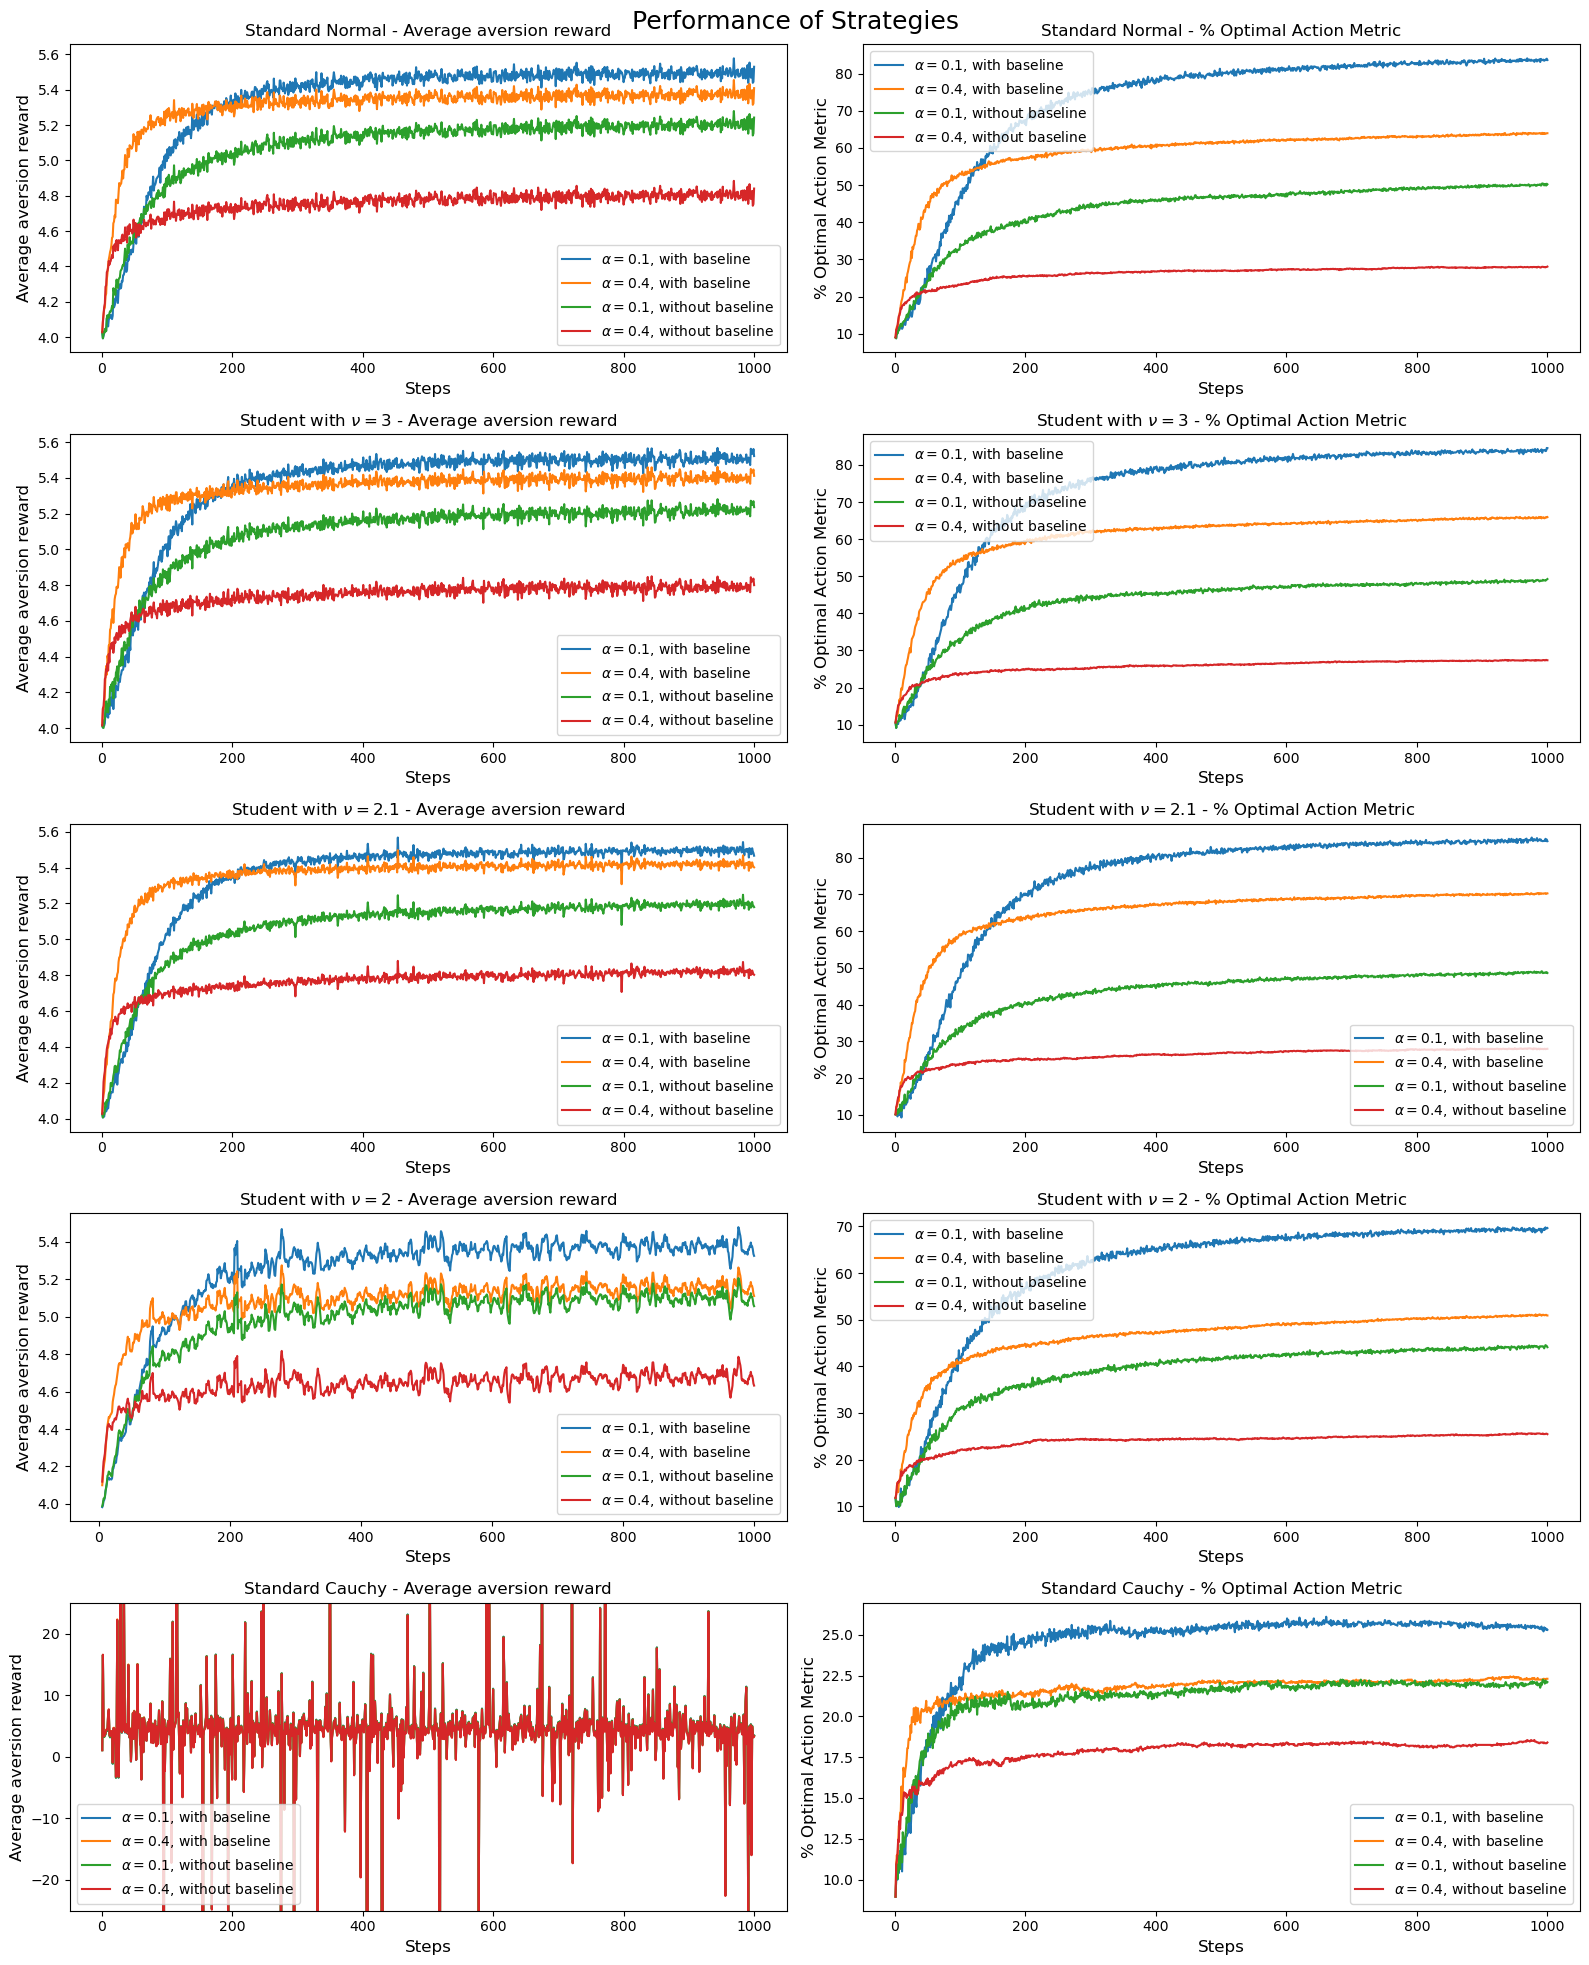
\includegraphics[width=1.1\linewidth]{Figures/experiments_classic/gradient_bandits/first.png}
    \caption{\label{fig:gradient_1}Значения средней награды и процента оптимального выбора для gradient bandits, сгруппировано по распределениям. Меньшее $\alpha$ и присутствие baseline приводят к лучшим результатам}
\end{figure}
\begin{figure}[ht!]
    \centering
    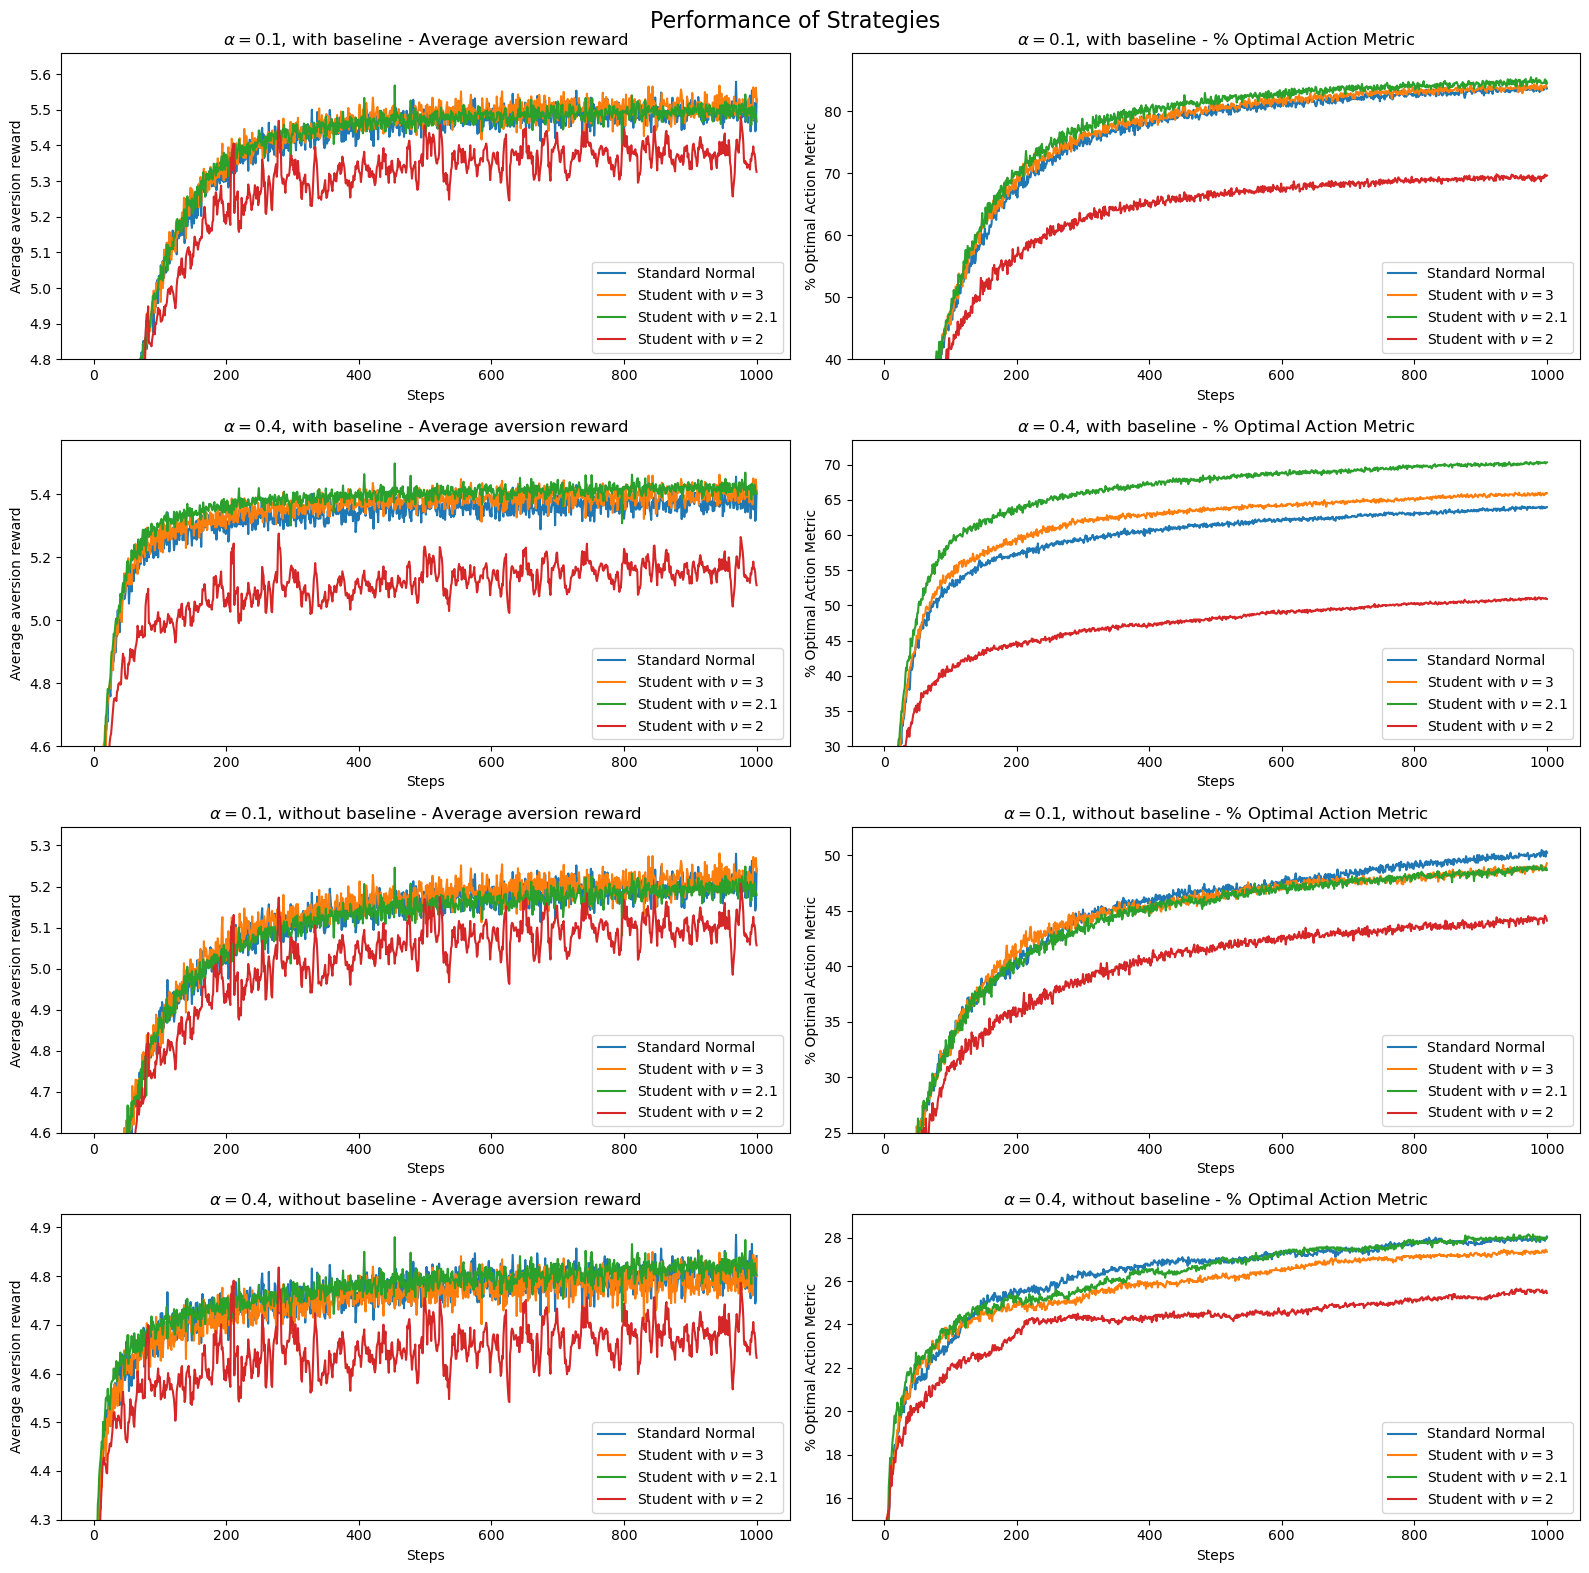
\includegraphics[width=1.1\linewidth]{Figures/experiments_classic/gradient_bandits/second.png}
    \caption{\label{fig:gradient_2}Значения средней награды и процента оптимального выбора для gradient bandits, сгруппировано по стратегиям. Заметно странное поведение метрик: когда есть baseline, значения для $t_{2.1}$ лучше, чем для $t_{3}$}.
\end{figure}

\section{Сравнение всех стратегий}

В целом, характерны следующие тенденции:
\begin{enumerate}
    \item У $t_2$ имеются резкие перепады в средней награде с сохранением тенденции к увеличению (или уменьшению для постоянного step-size). Это объясняется отсутсвием у $t_2$ дисперсии.
    \item Везде, кроме greedy стратегий и стратегий с постоянным step-size, занчения метрик для $t_{\infty}$ и $t_3$ почти совпадают, то есть стратегии одинаково применимы для этих двух распределений.
\end{enumerate}

Наконец, проанализируем графики со сравнениями всех стратегий. Для всех распределений лучшую среднюю награду и процент оптимальных действий выдает UCB. Хотя для $t_{\infty}$ жадная позитивная инициализация идет второй по итоговому значению и лишь немного уступает UCB, заметна тенденция падения относительно других стратегий максимального значения для жадной позитивной инициализации с постоянным step-size при уменьшающемся $\nu$. На всех графиках, кроме $t_1$, градиентные бандиты показывают себя немного лучше, чем $\epsilon$-greedy. Как уже было сказано, график средней награды для распределения Коши не имеет смысла, для процента оптимальных действий лучшие значения достигаются для $\epsilon$-greedy и UCB, при этом значения метрики для gradient bandits значительно падают относительно этих стратегий. Так происходит, поскольку baseline есть среднее по всем предыдущим шагам, что не сходится ни к какому значению при любом распределении выбора действий.

В целом UCB на всех распределениях показывает лучший или один из лучших результатов, что можно объяснить тем, что эта стратегия дает любому рычагу воможность быть выбранным, при этом эта вероятность быть выбранным уменьшается с увеличением числа шагов и при этом в меньшей степени привязана к матожиданию, как, например, gradient bandits. Так как так же дается ненулевая вероятность быть выбранным каждому рычагу, $\epsilon$-greedy и gradient bandits тоже дают хорошие результаты на $t_2, t_{2.1}, t_3, t_{\infty}$.

\begin{figure}[ht!]
    \centering
    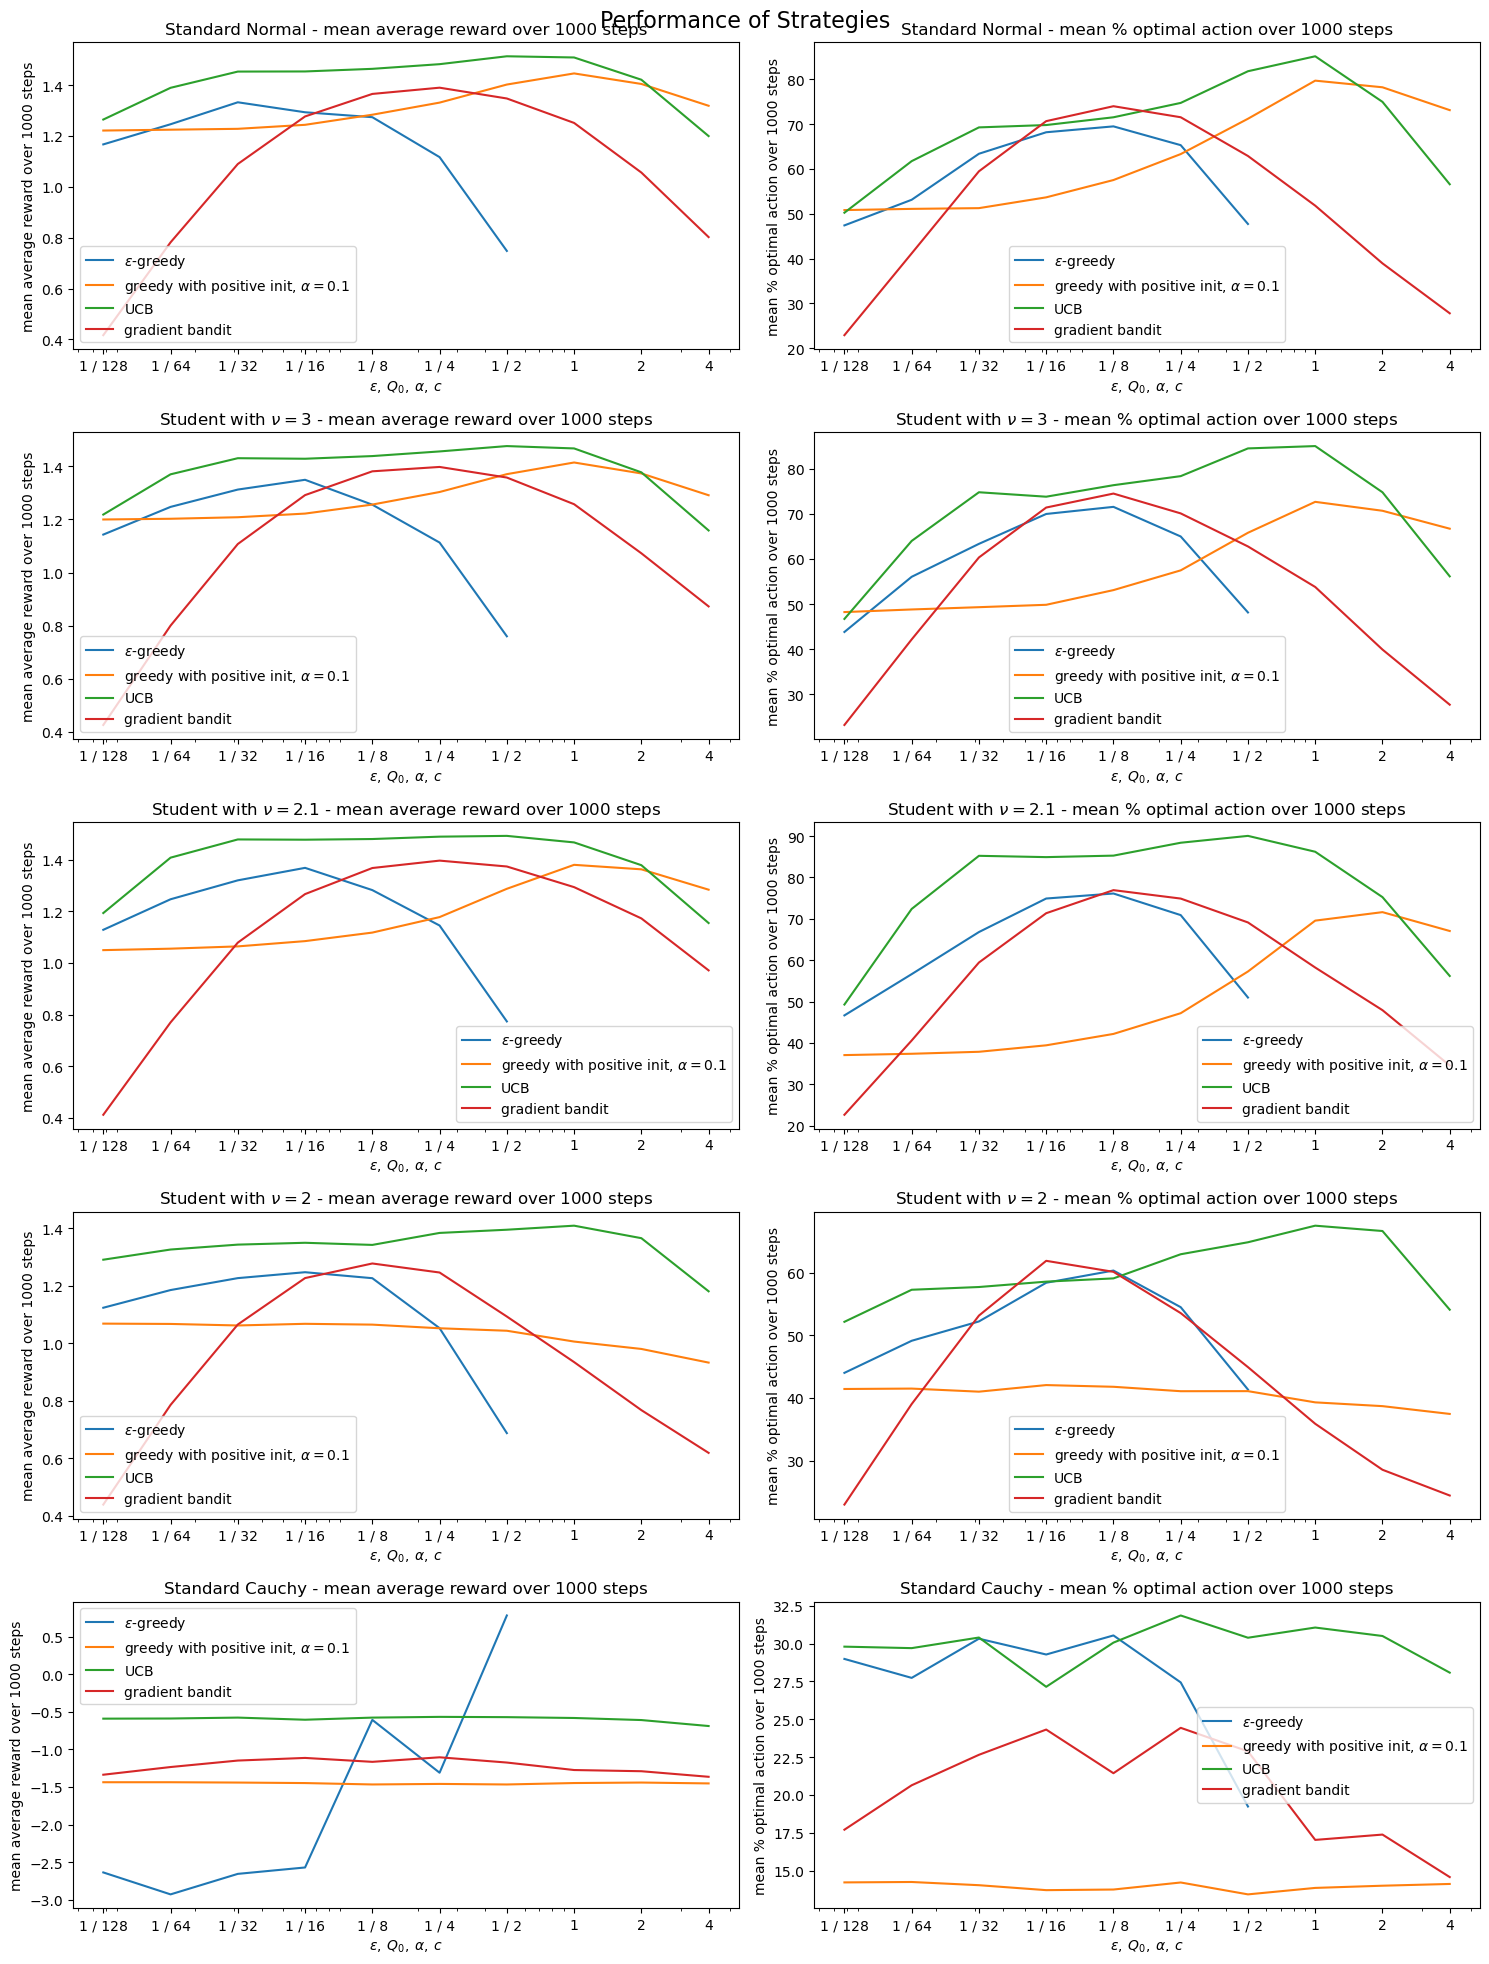
\includegraphics[width=1.1\linewidth]{experiments_classic/overall/overall.png}
    \caption{\label{fig:overall}Сравнение всех стратегий при варьировании гиперпараметров}
\end{figure}

\section{Выводы}

Проделанные эксперименты позволяют судить о том, что Gradient bandits, $\epsilon$-greedy и UCB -- стратегии показывают высокую эффективность на степенных распределениях. Так как UCB -- единственная из стратегий, показывающая высокую эффективность на всех метриках и всех распределениях, то эта стратегия, при условии, что существует способ адаптации доверительного интервала для дисперсии -- лучший кандидат на применение в задаче о многоруких бандитах с учетом отвращения к риску.